\documentclass[12pt, a4paper]{article}
\usepackage[a4paper, left=2cm, right=2cm, top=3cm, bottom=3cm]{geometry}

\usepackage[english]{babel}
\usepackage[utf8]{inputenc}
\usepackage{fancyhdr}

\usepackage{enumitem}
\usepackage{amsmath}
\usepackage{mathtools}
\usepackage{listings}

\usepackage{tikz}
\usetikzlibrary{arrows.meta,shapes.multipart}

\pagestyle{fancy}
\fancyhf{}
\lhead{Tutorium 02 \\ Abgabegruppe 01}
\chead{Blatt 03 \\ DatKom}
\rhead{Andrés Montoya, 405409 \\ Til Mohr, 405959}

\begin{document}

\begin{center}\fcolorbox{red}{yellow}{\begin{minipage}{35em}
	Bei uns war ursprünglich noch ein Dritter in unserer Abgabegruppe eingeteilt. Wir haben ihn vor über einer Woche versucht per E-Mail zu erreichen, leider erfolglos.\\
	Nach Ablauf der Anmeldefrist zu den Abgabegruppen haben wir gesehen, dass diese Person leider unsere Abgabegruppe verlassen hat.\\
	Bisher konnten wir noch keinen Dritten für unsere Abgabegruppe finden.\\
	Uns wurde auch seit dem letzten Blatt keine weitere Person zugeteilt.
\end{minipage}}\end{center}



\section*{Aufgabe 3.1}
Wir haben eine Grenzfrequenz $\operatorname{f}_{\text{grenz}} = 384 \text{kHz}$ gegeben. Die Abtastfrequenz soll nun mindestens doppelt so groß sein: 
$$\operatorname{f}_{\text{a}} \geq 2 \cdot \operatorname{f}_{\text{grenz}} \Rightarrow \operatorname{f}_{\text{a}} = 2 \cdot 384 \text{kHz} = 768 \text{kHz}$$
Es wird also eine Datenrate von mind. $768 \text{kHz} \cdot 32 \text{Bit} = 24576 \frac{\text{Bit}}{\text{s}}$ benötigt.



\section*{Aufagbe 3.2}
\begin{enumerate}[label=\alph*)]
	\item	Mobilfunkgerät $1$: $1,1,1 \mapsto -a,-a,-a = -1,1,-1,1, -1,1,-1,1, -1,1,-1,1$\\
			Mobilfunkgerät $2$: $1,0,0 \mapsto -b,b,b = -1,1,1,-1, 1,-1,-1,1, 1,-1,-1,1$
	
	\item	$1,1,-1,-1, -1,-1,1,1, -1,-1,1,1$
	
	\item	Es erscheint dann der Basisstation, als würden beide Mobilfunkgeräte zu unterschiedlichen Zeiten senden, weshalb die Signalfolgen von beiden sich nicht bezogen auf die Codes optimal überlagern, weshalb die Basistation die Daten nicht einsehen kann.
\end{enumerate}



\section*{Aufgabe 3.3}
\begin{enumerate}[label=\alph*)]
	\item	Gestuffte Bits sind unterstrichen:
			$$01111110 011111\underline{0}10 01000111 11000111 11\underline{0}100000 01111110$$
	
	\item	Gestuffte Character sind unterstrichen:
			$$11100000 01111110 01111110 01000111 11000111 \underline{11100000} 11100000 11100000 01111110$$
	
	\item	Im schlimmsten Fall überträgt man bei Bit-Stuffing genau seine Bit-Folge. Abgesehen von der Bit-Folge, die man vor und nach den Daten hinzufügt, muss man noch eine 0 stopfen.\\
			Im schlimmsten Fall überträgt man bei Character-Stuffing genau sein DLE. Abgesehen von den zwei DLE, einem STX und einem ETX, die man noch hinzufügen muss, muss man noch ein DLE stopfen.
\end{enumerate}

\newpage

\section*{Aufgabe 3.4}
\begin{itemize}
	\item[$40$]		$$40 \text{Byte} = 40 \cdot 8 \text{Bit} = 320 \text{Bit}$$
					$$\text{ PER } = 1 - (1-10^{-5})^{320} \approx 1 - 0.996805098594 = 0.00319490140594$$
	
	\item[$1400$]	$$1400 \text{Byte} = 1400 \cdot 8 \text{Bit} = 11200 \text{Bit}$$
					$$\text{ PER } = 1 - (1-10^{-5})^{11200} \approx 1 - 0.894043756833 = 0.105956243167$$
\end{itemize}



\section*{Aufgabe 3.5}
\begin{enumerate}[label=\alph*)]
	\item	Nun können eine ungerade Anzahl an Fehlern erkannt werden an sowohl den geraden als auch den ungeraden Positionen. Korrigiert können jedoch keine Fehler werden, da hierzu die Positionen wichtig sind, und dazu zu wenig Information gegeben ist (gerade $\leftrightarrow$ ungerade: reicht nur aus, wenn 2 Bits übertragen werden).
	
	\item	Längsparität:
			$$01100$$
			Querparität:
			$$010010$$
\end{enumerate}

\newpage

\section*{Aufgabe 3.6}
\begin{enumerate}[label=\alph*)]
	\item	$101000110000 \div 10101$ liefert uns den Rest $1101$.\\
			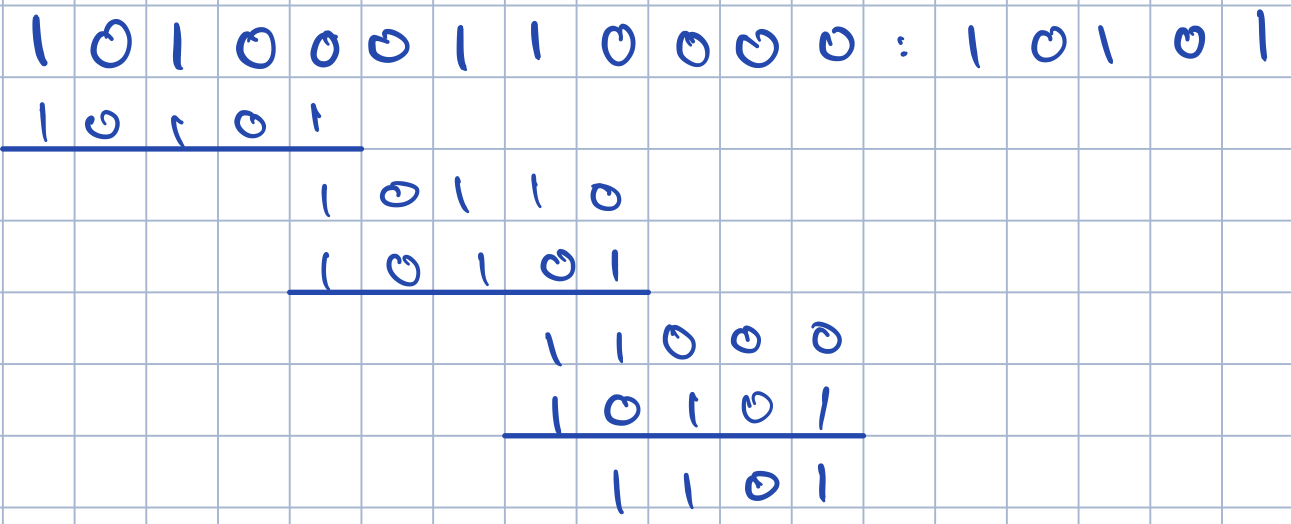
\includegraphics[scale=0.6]{3.6_a.png}
	
	\item	$011111000101 \div 10101$ liefert uns einen Rest $\neq 0$. Daher ist ein Fehler aufgetreten.\\
			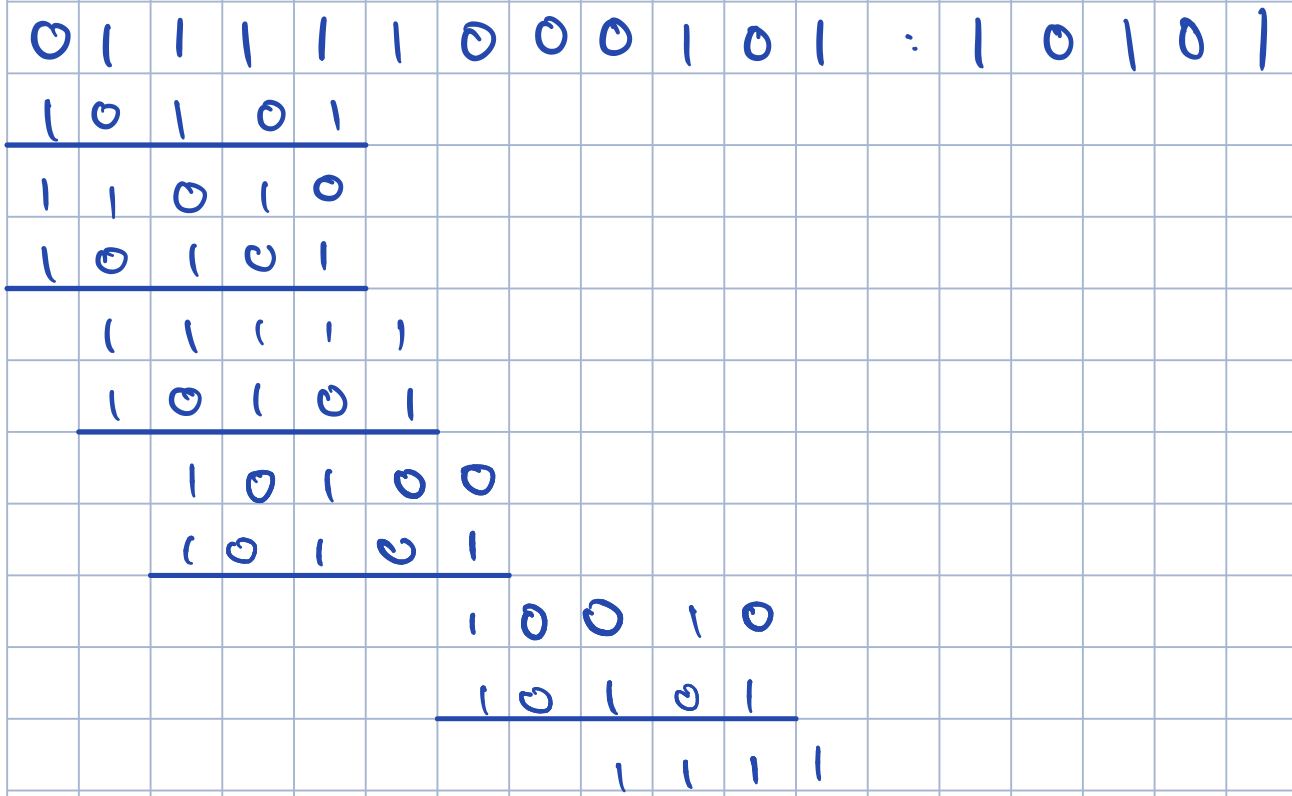
\includegraphics[scale=0.6]{3.6_b.png}
	
	\item	
\end{enumerate}


\end{document}